% IEEE Communications Letters style manuscript (two-column, double-anonymous).
% Every numeric value is a macro from paper/numbers.tex, generated from results/
% by scripts/make_numbers.py (AGENTS.md rule 1).  Do not type numbers inline.
%
% Alternative title:
%   The Burden Falls on the Higher Constellation: Geographic Incidence of
%   47 CFR 25.261 for Co-Frequency NGSO User Downlinks
\documentclass[journal,10pt]{IEEEtran}

\usepackage{graphicx}
\usepackage{amsmath}
\usepackage{booktabs}
\usepackage{url}
\usepackage[hidelinks]{hyperref}

\graphicspath{{figures/}}

% AUTOGENERATED by scripts/make_numbers.py -- do not edit by hand.
% Every macro below is read from results/ (AGENTS.md rule 1).
% Newest run per experiment:
% SharedFreqGhz <- results/e1_event_rate_20261018T012116Z_seed0/
% EventNPhasings <- results/e1_event_rate_20261018T012116Z_seed0/
% ThetaColoPeakPct <- results/e1_event_rate_20261018T012116Z_seed0/
% ThetaColoPeakLat <- results/e1_event_rate_20261018T012116Z_seed0/
% ThetaColoEquatorPct <- results/e1_event_rate_20261018T012116Z_seed0/
% ThetaWorstPeakPct <- results/e1_event_rate_20261018T012116Z_seed0/
% UnresGeomWithDivPct <- results/e2_diversity_20261019T145056Z_seed0/
% MinElevLowDeg <- results/e2_diversity_20261019T145056Z_seed0/
% MinElevHighDeg <- results/e2_diversity_20261019T145056Z_seed0/
% MinElevPeakLowPct <- results/e2_diversity_20261019T145056Z_seed0/
% MinElevPeakHighPct <- results/e2_diversity_20261019T145056Z_seed0/
% CapUnresMaxPct <- results/e3_capacity_diversity_20261018T012933Z_seed0/
% CapUnresCondNbeamEight <- results/e3_capacity_diversity_20261018T012933Z_seed0/
% CapUnresCondNbeamSixteen <- results/e3_capacity_diversity_20261018T012933Z_seed0/
% CapUnresCondNbeamThirtyTwo <- results/e3_capacity_diversity_20261018T012933Z_seed0/
% OnewebEirpDbw <- results/e4_dtt_20261019T143641Z_seed0/
% BindFilWorstPct <- results/e4_dtt_20261019T143641Z_seed0/
% BindFilColoPct <- results/e4_dtt_20261019T143641Z_seed0/
% BindFilWorstLat <- results/e4_dtt_20261019T143641Z_seed0/
% BindWithDivPct <- results/e4_dtt_20261019T143641Z_seed0/
% BindFilStarWorstPct <- results/e4_dtt_20261019T143641Z_seed0/
% BindFilStarColoPct <- results/e4_dtt_20261019T143641Z_seed0/
% BaselineCnMedOneDb <- results/e4_dtt_20261019T143641Z_seed0/
% BaselineCnPTenOneDb <- results/e4_dtt_20261019T143641Z_seed0/
% BaselineAvailOneMinPct <- results/e4_dtt_20261019T143641Z_seed0/
% CalRefCnMedDb <- results/e4_dtt_20261019T143641Z_seed0/
% CalRefCnPTenDb <- results/e4_dtt_20261019T143641Z_seed0/
% QualOneCases <- results/e4_dtt_20261019T143641Z_seed0/
% QualOneTotal <- results/e4_dtt_20261019T143641Z_seed0/
% BaselineCnMedStarDb <- results/e4_dtt_20261019T143641Z_seed0/
% BaselineCnPTenStarDb <- results/e4_dtt_20261019T143641Z_seed0/
% BaselineAvailStarMinPct <- results/e4_dtt_20261019T143641Z_seed0/
% QualStarCases <- results/e4_dtt_20261019T143641Z_seed0/
% QualStarTotal <- results/e4_dtt_20261019T143641Z_seed0/
% DegrFilWorstPctFourFive <- results/e4_dtt_20261019T143641Z_seed0/
% DegrFilWorstPctSixZero <- results/e4_dtt_20261019T143641Z_seed0/
% DegrFilWorstPctSevenFive <- results/e4_dtt_20261019T143641Z_seed0/
% DegrFilMaxPct <- results/e4_dtt_20261019T143641Z_seed0/
% DegrFilMaxCi <- results/e4_dtt_20261019T143641Z_seed0/
% DegrFilColoPct <- results/e4_dtt_20261019T143641Z_seed0/
% DegrFilColoCi <- results/e4_dtt_20261019T143641Z_seed0/
% UnavailIncColoPct <- results/e4_dtt_20261019T143641Z_seed0/
% UnavailIncColoCi <- results/e4_dtt_20261019T143641Z_seed0/
% DegrFilStarPct <- results/e4_dtt_20261019T143641Z_seed0/
% UnavailIncPct <- results/e4_dtt_20261019T143641Z_seed0/
% UnavailIncCi <- results/e4_dtt_20261019T143641Z_seed0/
% NStarlinkRaw <- results/e5_as_deployed_20261019T144239Z_seed0/
% NStarlinkOp <- results/e5_as_deployed_20261019T144239Z_seed0/
% NOnewebRaw <- results/e5_as_deployed_20261019T144239Z_seed0/
% NOnewebOp <- results/e5_as_deployed_20261019T144239Z_seed0/
% NStartTimes <- results/e5_as_deployed_20261019T144239Z_seed0/
% BindDepWorstPct <- results/e5_as_deployed_20261019T144239Z_seed0/
% BindDepWorstCi <- results/e5_as_deployed_20261019T144239Z_seed0/
% BindDepWorstLat <- results/e5_as_deployed_20261019T144239Z_seed0/
% BindDepColoPct <- results/e5_as_deployed_20261019T144239Z_seed0/
% BindDepColoCi <- results/e5_as_deployed_20261019T144239Z_seed0/
% BindDepColoLat <- results/e5_as_deployed_20261019T144239Z_seed0/
% DegrDepWorstPctFourFive <- results/e5_as_deployed_20261019T144239Z_seed0/
% DegrDepWorstPctSixZero <- results/e5_as_deployed_20261019T144239Z_seed0/
% DegrDepWorstPctSevenFive <- results/e5_as_deployed_20261019T144239Z_seed0/
% DegrDepMaxPct <- results/e5_as_deployed_20261019T144239Z_seed0/
% DegrDepMaxCi <- results/e5_as_deployed_20261019T144239Z_seed0/
% UnavailIncDepPct <- results/e5_as_deployed_20261019T144239Z_seed0/
% UnavailIncDepCi <- results/e5_as_deployed_20261019T144239Z_seed0/
% DegrDepColoPct <- results/e5_as_deployed_20261019T144239Z_seed0/
% DegrDepColoCi <- results/e5_as_deployed_20261019T144239Z_seed0/
% UnavailIncColoDepPct <- results/e5_as_deployed_20261019T144239Z_seed0/
% UnavailIncColoDepCi <- results/e5_as_deployed_20261019T144239Z_seed0/
% BaselineAvailOneDepPct <- results/e5_as_deployed_20261019T144239Z_seed0/
% BindDepStarWorstPct <- results/e5_as_deployed_20261019T144239Z_seed0/
% BindMinApertureDepPct <- results/e5_as_deployed_20261019T144239Z_seed0/
% BindMaxApertureDepPct <- results/e5_as_deployed_20261019T144239Z_seed0/
% DegrDepStarPct <- results/e5_as_deployed_20261019T144239Z_seed0/
% DegrWithDivPct <- results/e5_as_deployed_20261019T144239Z_seed0/
% GeomRatioEquator <- results/e5_as_deployed_20261019T144239Z_seed0/
% BindRatioEquator <- results/e5_as_deployed_20261019T144239Z_seed0/
% BindRatioPeak <- results/e5_as_deployed_20261019T144239Z_seed0/
% EirpHeadDiam <- results/e6_eirp_sweep_20261019T144513Z_seed0/
% EirpSweepValues <- results/e6_eirp_sweep_20261019T144513Z_seed0/
% EirpFwdInvariantPct <- results/e6_eirp_sweep_20261019T144513Z_seed0/
% EirpFwdColoPct <- results/e6_eirp_sweep_20261019T144513Z_seed0/
% EirpFwdUnresPct <- results/e6_eirp_sweep_20261019T144513Z_seed0/
% EirpFwdBaseAvailPct <- results/e6_eirp_sweep_20261019T144513Z_seed0/
% EirpRevMinPct <- results/e6_eirp_sweep_20261019T144513Z_seed0/
% EirpRevMaxPct <- results/e6_eirp_sweep_20261019T144513Z_seed0/
% EirpDegrMinPct <- results/e6_eirp_sweep_20261019T144513Z_seed0/
% EirpDegrMaxPct <- results/e6_eirp_sweep_20261019T144513Z_seed0/
% EirpDegrMinCi <- results/e6_eirp_sweep_20261019T144513Z_seed0/
% EirpDegrMaxCi <- results/e6_eirp_sweep_20261019T144513Z_seed0/
% EirpDegrAtCalPct <- results/e6_eirp_sweep_20261019T144513Z_seed0/
% EirpDegrAtCalCi <- results/e6_eirp_sweep_20261019T144513Z_seed0/
% EirpRevAtCalPct <- results/e6_eirp_sweep_20261019T144513Z_seed0/
% EirpRevHoldMinDbw <- results/e6_eirp_sweep_20261019T144513Z_seed0/
% EirpRevHoldPct <- results/e6_eirp_sweep_20261019T144513Z_seed0/
% EirpPrimFwdWorstPct <- results/e6_eirp_sweep_20261019T144513Z_seed0/
% EirpPrimFwdUnresPct <- results/e6_eirp_sweep_20261019T144513Z_seed0/
% EirpPrimFwdDegrPct <- results/e6_eirp_sweep_20261019T144513Z_seed0/
% EirpPrimFwdDegrCi <- results/e6_eirp_sweep_20261019T144513Z_seed0/
% EirpPrimColoPct <- results/e6_eirp_sweep_20261019T144513Z_seed0/
% EirpPrimRevWorstPct <- results/e6_eirp_sweep_20261019T144513Z_seed0/
% EirpLowFwdWorstPct <- results/e6_eirp_sweep_20261019T144513Z_seed0/
% EirpLowFwdUnresPct <- results/e6_eirp_sweep_20261019T144513Z_seed0/
% EirpLowFwdDegrPct <- results/e6_eirp_sweep_20261019T144513Z_seed0/
% EirpLowFwdDegrCi <- results/e6_eirp_sweep_20261019T144513Z_seed0/
% EirpLowColoPct <- results/e6_eirp_sweep_20261019T144513Z_seed0/
% EirpLowRevWorstPct <- results/e6_eirp_sweep_20261019T144513Z_seed0/
% EirpDpCommonFwdWorstPct <- results/e6_eirp_sweep_20261019T144513Z_seed0/
% EirpDpCommonFwdUnresPct <- results/e6_eirp_sweep_20261019T144513Z_seed0/
% EirpDpCommonFwdDegrPct <- results/e6_eirp_sweep_20261019T144513Z_seed0/
% EirpDpCommonFwdDegrCi <- results/e6_eirp_sweep_20261019T144513Z_seed0/
% EirpDpCommonColoPct <- results/e6_eirp_sweep_20261019T144513Z_seed0/
% EirpDpCommonRevWorstPct <- results/e6_eirp_sweep_20261019T144513Z_seed0/
% EirpCnCalFwdWorstPct <- results/e6_eirp_sweep_20261019T144513Z_seed0/
% EirpCnCalFwdUnresPct <- results/e6_eirp_sweep_20261019T144513Z_seed0/
% EirpCnCalFwdDegrPct <- results/e6_eirp_sweep_20261019T144513Z_seed0/
% EirpCnCalFwdDegrCi <- results/e6_eirp_sweep_20261019T144513Z_seed0/
% EirpCnCalColoPct <- results/e6_eirp_sweep_20261019T144513Z_seed0/
% EirpCnCalRevWorstPct <- results/e6_eirp_sweep_20261019T144513Z_seed0/
% EirpPfdFwdWorstPct <- results/e6_eirp_sweep_20261019T144513Z_seed0/
% EirpPfdFwdUnresPct <- results/e6_eirp_sweep_20261019T144513Z_seed0/
% EirpPfdFwdDegrPct <- results/e6_eirp_sweep_20261019T144513Z_seed0/
% EirpPfdFwdDegrCi <- results/e6_eirp_sweep_20261019T144513Z_seed0/
% EirpPfdColoPct <- results/e6_eirp_sweep_20261019T144513Z_seed0/
% EirpPfdRevWorstPct <- results/e6_eirp_sweep_20261019T144513Z_seed0/

\newcommand{\DttThreshold}{0.06}
\newcommand{\DttLongTerm}{0.03}
\newcommand{\LongTermFraction}{0.004}
\newcommand{\DegradeLimitPct}{3}
\newcommand{\UnavailLimitPct}{0.4}
\newcommand{\SharedFreqGhz}{11.7}
\newcommand{\EventNPhasings}{8}
\newcommand{\ThetaColoPeakPct}{0.47}
\newcommand{\ThetaColoPeakLat}{50}
\newcommand{\ThetaColoEquatorPct}{0.21}
\newcommand{\ThetaWorstPeakPct}{2.52}
\newcommand{\UnresGeomWithDivPct}{0.000}
\newcommand{\MinElevLowDeg}{20}
\newcommand{\MinElevHighDeg}{35}
\newcommand{\MinElevPeakLowPct}{0.47}
\newcommand{\MinElevPeakHighPct}{0.47}
\newcommand{\CapUnresMaxPct}{0.0012}
\newcommand{\CapUnresCondNbeamEight}{0.0004445}
\newcommand{\CapUnresCondNbeamSixteen}{0.0003074}
\newcommand{\CapUnresCondNbeamThirtyTwo}{0.0001908}
\newcommand{\OnewebEirpDbw}{10.6}
\newcommand{\BindFilWorstPct}{100.00}
\newcommand{\BindFilColoPct}{73.04}
\newcommand{\BindFilWorstLat}{0}
\newcommand{\BindWithDivPct}{100.000}
\newcommand{\BindFilStarWorstPct}{47.17}
\newcommand{\BindFilStarColoPct}{14.08}
\newcommand{\BaselineCnMedOneDb}{12.4}
\newcommand{\BaselineCnPTenOneDb}{10.7}
\newcommand{\BaselineAvailOneMinPct}{100}
\newcommand{\CalRefCnMedDb}{15.4}
\newcommand{\CalRefCnPTenDb}{14.7}
\newcommand{\QualOneCases}{84}
\newcommand{\QualOneTotal}{84}
\newcommand{\BaselineCnMedStarDb}{25.6}
\newcommand{\BaselineCnPTenStarDb}{24.3}
\newcommand{\BaselineAvailStarMinPct}{100}
\newcommand{\QualStarCases}{84}
\newcommand{\QualStarTotal}{84}
\newcommand{\DegrFilWorstPctFourFive}{45.99}
\newcommand{\DegrFilWorstPctSixZero}{40.91}
\newcommand{\DegrFilWorstPctSevenFive}{37.41}
\newcommand{\DegrFilMaxPct}{45.99}
\newcommand{\DegrFilMaxCi}{0.47}
\newcommand{\DegrFilColoPct}{10.37}
\newcommand{\DegrFilColoCi}{0.17}
\newcommand{\UnavailIncColoPct}{1.872}
\newcommand{\UnavailIncColoCi}{0.041}
\newcommand{\DegrFilStarPct}{2.63}
\newcommand{\UnavailIncPct}{9.571}
\newcommand{\UnavailIncCi}{0.307}
\newcommand{\NStarlinkRaw}{10651}
\newcommand{\NStarlinkOp}{9737}
\newcommand{\NOnewebRaw}{651}
\newcommand{\NOnewebOp}{648}
\newcommand{\NStartTimes}{8}
\newcommand{\BindDepWorstPct}{100.00}
\newcommand{\BindDepWorstCi}{0.00}
\newcommand{\BindDepWorstLat}{0}
\newcommand{\BindDepColoPct}{83.94}
\newcommand{\BindDepColoCi}{0.09}
\newcommand{\BindDepColoLat}{50}
\newcommand{\DegrDepWorstPctFourFive}{58.32}
\newcommand{\DegrDepWorstPctSixZero}{52.65}
\newcommand{\DegrDepWorstPctSevenFive}{48.55}
\newcommand{\DegrDepMaxPct}{58.32}
\newcommand{\DegrDepMaxCi}{0.13}
\newcommand{\UnavailIncDepPct}{12.741}
\newcommand{\UnavailIncDepCi}{0.096}
\newcommand{\DegrDepColoPct}{12.52}
\newcommand{\DegrDepColoCi}{0.05}
\newcommand{\UnavailIncColoDepPct}{1.860}
\newcommand{\UnavailIncColoDepCi}{0.074}
\newcommand{\BaselineAvailOneDepPct}{100}
\newcommand{\BindDepStarWorstPct}{39.89}
\newcommand{\BindMinApertureDepPct}{100.00}
\newcommand{\BindMaxApertureDepPct}{100.00}
\newcommand{\DegrDepStarPct}{2.23}
\newcommand{\DegrWithDivPct}{58.318}
\newcommand{\GeomRatioEquator}{1.51}
\newcommand{\BindRatioEquator}{1.0}
\newcommand{\BindRatioPeak}{1.0}
\newcommand{\EirpHeadDiam}{0.45}
\newcommand{\EirpSweepValues}{12.1, 12.7, 15.68}
\newcommand{\EirpFwdInvariantPct}{100.00}
\newcommand{\EirpFwdColoPct}{84.32}
\newcommand{\EirpFwdUnresPct}{100.00}
\newcommand{\EirpFwdBaseAvailPct}{100}
\newcommand{\EirpRevMinPct}{4.31}
\newcommand{\EirpRevMaxPct}{72.43}
\newcommand{\EirpDegrMinPct}{34.25}
\newcommand{\EirpDegrMaxPct}{75.22}
\newcommand{\EirpDegrMinCi}{0.15}
\newcommand{\EirpDegrMaxCi}{0.18}
\newcommand{\EirpDegrAtCalPct}{58.53}
\newcommand{\EirpDegrAtCalCi}{0.21}
\newcommand{\EirpRevAtCalPct}{40.01}
\newcommand{\EirpRevHoldMinDbw}{0.2}
\newcommand{\EirpRevHoldPct}{4.31}
\newcommand{\EirpPrimFwdWorstPct}{100.00}
\newcommand{\EirpPrimFwdUnresPct}{100.00}
\newcommand{\EirpPrimFwdDegrPct}{58.53}
\newcommand{\EirpPrimFwdDegrCi}{0.21}
\newcommand{\EirpPrimColoPct}{84.32}
\newcommand{\EirpPrimRevWorstPct}{40.01}
\newcommand{\EirpLowFwdWorstPct}{100.00}
\newcommand{\EirpLowFwdUnresPct}{100.00}
\newcommand{\EirpLowFwdDegrPct}{42.87}
\newcommand{\EirpLowFwdDegrCi}{0.19}
\newcommand{\EirpLowColoPct}{56.78}
\newcommand{\EirpLowRevWorstPct}{40.01}
\newcommand{\EirpDpCommonFwdWorstPct}{100.00}
\newcommand{\EirpDpCommonFwdUnresPct}{100.00}
\newcommand{\EirpDpCommonFwdDegrPct}{45.43}
\newcommand{\EirpDpCommonFwdDegrCi}{0.20}
\newcommand{\EirpDpCommonColoPct}{61.28}
\newcommand{\EirpDpCommonRevWorstPct}{40.01}
\newcommand{\EirpCnCalFwdWorstPct}{100.00}
\newcommand{\EirpCnCalFwdUnresPct}{100.00}
\newcommand{\EirpCnCalFwdDegrPct}{75.22}
\newcommand{\EirpCnCalFwdDegrCi}{0.18}
\newcommand{\EirpCnCalColoPct}{84.32}
\newcommand{\EirpCnCalRevWorstPct}{4.31}
\newcommand{\EirpPfdFwdWorstPct}{100.00}
\newcommand{\EirpPfdFwdUnresPct}{100.00}
\newcommand{\EirpPfdFwdDegrPct}{66.21}
\newcommand{\EirpPfdFwdDegrCi}{0.17}
\newcommand{\EirpPfdColoPct}{85.82}
\newcommand{\EirpPfdRevWorstPct}{72.43}


\begin{document}

\title{Frequent In-Line Events, Conditional Compliance:\\
Satellite Diversity Decides the FCC's NGSO Sharing Limits}

% Double-anonymous submission: no author or affiliation information.
\author{Anonymous Submission}

\maketitle

\begin{abstract}
Under 47 CFR~25.261, co-frequency non-geostationary (NGSO) systems split the band
while the victim's noise-temperature increment $\Delta T/T$ exceeds
\DttThresholdPct\%, and \S\,25.261(d) bounds the resulting throughput
degradation (\DegradeLimitPct\%) and availability change (\UnavailLimitPct\%).
We measure these criteria versus earth-station latitude for the only
co-frequency Ku user-downlink pair among Starlink, OneWeb, and Kuiper, using a
filed Walker geometry and an as-deployed CelesTrak snapshot, with Starlink held
at the 47 CFR~25.208(b) PFD limit. In-line events are frequent: the OneWeb-victim
time fraction peaks at \BindDepWorstPct$\pm$\BindDepWorstCi\% as deployed,
\BurdenRatioDep$\times$ the Starlink-victim peak. Without satellite diversity,
both \S\,25.261(d) limits are exceeded at the PFD limit
(\DegrDepMaxPct$\pm$\DegrDepMaxCi\% and
\UnavailIncDepPct$\pm$\UnavailIncDepCi\%) and still \PfdOffsetThreeDb~dB below
it; \PfdOffsetSixDb~dB below it the throughput limit is met and the availability
change is not distinguishable from its limit. With diversity, both limits are met
in every case studied. Compliance therefore depends on a mitigation the rule does
not mention, and the burden falls on the higher-altitude, lower-EIRP system.
\end{abstract}

\begin{IEEEkeywords}
NGSO, spectrum sharing, in-line interference, 47 CFR 25.261, satellite
diversity, Starlink, OneWeb.
\end{IEEEkeywords}

\section{Introduction}
\IEEEPARstart{C}{o-frequency} sharing between low-Earth-orbit broadband
constellations is governed in the United States by 47 CFR~25.261~\cite{cfr25261}.
Absent coordination, \S\,25.261(c) divides the commonly authorized band among
systems of the same processing round whenever interference from the other system
raises a receiver's $\Delta T/T$ above \DttThresholdPct\%, for as long as the
excess lasts~\cite{fcc2329}; this threshold \emph{defines} the in-line event.
Between processing rounds, \S\,25.261(d)~\cite{fcc24117} protects earlier-round
systems: a later-round system may cause no more than \DegradeLimitPct\%
time-weighted average degraded throughput and no more than \UnavailLimitPct\%
absolute change in link availability, for links with at least
\RuleBaselineAvailPct\% baseline availability at a C/N threshold of
\CnGateDb~dB. A separate, recent proceeding replaces the
equivalent-PFD framework for NGSO--GSO sharing~\cite{fcc2626}; it does not change
the NGSO--NGSO criteria studied here.

Prior work has asked whether interference among dense NGSO constellations is a
practical concern~\cite{braun2019} and analyzed the feasibility of in-band
coexistence of dense LEO systems~\cite{kim2025}. Neither evaluates the FCC's own
criteria. This letter does so for a real co-frequency pair: it resolves the
\S\,25.261(c) event and the \S\,25.261(d) limits by latitude and direction, for
filed and as-deployed geometry, with and without satellite diversity, and shows
that compliance hinges on diversity, which the rule does not mention.

\section{System Model}
\label{sec:model}

\emph{Geometry.} Starlink, OneWeb, and Kuiper are modelled as filed Walker-Delta
shells propagated with a two-body model plus $J_2$ secular drift, over
\EventNPhasings\ independent constellation phasings. The as-deployed geometry is a
CelesTrak snapshot~\cite{celestrak} (\NStarlinkRaw\ Starlink and \NOnewebRaw\
OneWeb objects, filtered to \NStarlinkOp\ and \NOnewebOp\ at operational
altitude) over \NStartTimes\ independent start times. Earth stations lie at
latitudes \LatMinDeg--\LatMaxDeg$^\circ$ in \LatStepDeg$^\circ$ steps on
\NLongitudes\ meridians, with a \StationMinElevDeg$^\circ$ minimum elevation; each
station is served by the highest-elevation visible satellite of its system.

\emph{Co-frequency overlap.} Only ordered pairs that share spectrum on the same
link type are screened. In the user downlink this leaves one pair, Starlink and
OneWeb in \SharedBandLoGhz--\SharedBandHiGhz~GHz, coupled at the band centre
\SharedFreqGhz~GHz; Kuiper's user downlink is in Ka band and does not overlap.

\emph{Criterion.} An event occurs while $\Delta T/T = I/N > \DttThreshold$
($I/N > \InThresholdDb$~dB), with $N = kT_{\text{sys}}B$ and $I$ the aggregate
received interference~\cite{cfr25261}. The victim receive gain follows ITU-R
S.1428~\cite{itu1428}; interferer off-axis emission follows ITU-R
S.1528~\cite{itu1528}. Three interferer aggregates are computed. \emph{Realistic}
(the main result): the interfering system's serving satellite points its main beam
at the site and every other visible interfering satellite contributes through its
S.1528 sidelobe. \emph{Co-located}: the serving satellite alone. \emph{Upper
bound}: every visible interfering satellite at peak EIRP, used only as a bound.

\emph{Interferer power.} Starlink Ku is PFD-constant, as it reduces power to hold
the surface PFD while steering: its EIRP density is set so that the PFD at the
\PfdAnchorElevDeg$^\circ$ service edge equals the 47 CFR~25.208(b) limit of
\PfdLimitDbw~dBW/m$^2$/MHz~\cite{cfr25208} (model value \PrimaryPfdDbw). As a
cross-check, the top of the filed EIRP range (\StarlinkFiledTopDbw~dBW/MHz after
conversion from the per-4-kHz unit) gives \FiledPfdDbw~dBW/m$^2$/MHz, within
\FiledPfdOffsetDb~dB of the limit. Section~25.208(b) covers only
\PfdScopeLoGhz--\PfdScopeHiGhz~GHz, whereas the shared band is
\SharedBandLoGhz--\SharedBandHiGhz~GHz; the limit is therefore an anchor for the
lower part of the band, and its relaxation is tested in Section~\ref{sec:results}.
OneWeb is constant-EIRP at \OnewebEirpDbw~dBW/MHz~\cite{delportillo2019}.

\emph{25.261(d) metrics and diversity.} Throughput is the Shannon rate with a
\ImplMarginDb~dB implementation margin; availability is the fraction of time with
C/N~$\ge \CnGateDb$~dB, and the limits apply only to links with baseline
availability of at least \RuleBaselineAvailPct\%. With satellite diversity the
victim may switch to any other visible satellite of its own system; diversity is
unlimited. \emph{Aggregation.} Every \S\,25.261(d) number below is the worst
qualifying station per replication (phasing or start time), averaged across
replications, with a \CiPct\% $t$-interval; a limit is \emph{exceeded} only if
the whole interval lies above it and \emph{met} only if it lies below.

\section{Analytic Approximation}
\label{sec:analytic}
For a PFD-constant interferer, $I/N$ depends on the victim's off-axis angle
$\theta$ alone, so the event reduces to $\theta < \theta^{*}$ with
$G_{\text{rx}}(\theta^{*}) = I/N|_{\text{thr}} + N - \text{PFD} -
10\log_{10}(\lambda^2/4\pi)$. In the S.1428 envelope $G = 32 - 25\log_{10}\theta$
($1^\circ$--$48^\circ$) the aperture cancels, giving
$\theta^{*} = \AnalyticThetaStarDeg^\circ$ for the OneWeb victim, with a spread of
\AnalyticThetaSpreadDeg$^\circ$ across \EirpHeadDiam--\AperMaxM~m apertures.
The co-located event probability is then $P = v_A v_B\,\Pr\{\angle(\hat
u_A,\hat u_B) < \theta^{*}\}$, where $v = 1 - e^{-n}$ is the probability that a
system has a satellite in view ($n$ the mean visible count) and each serving
direction is the nearest of $n$ satellites uniform in the ground footprint,
mapped to the look angle. The two serving directions are independent: feeding
the simulated marginals into the separation integral reproduces the simulated
separation probability within \DiagnosisIndepMaxErrPct\ percentage points (pp),
whereas a marginal uniform in the look-angle cap was in error by up to
\DiagnosisOldMaxErrPct~pp. Against the simulated co-located as-filed curve the
model is within \AnalyticMaxAbsErrPct~pp (signed error \AnalyticSignedMinPct\ to
\AnalyticSignedMaxPct~pp). The error varies with latitude: the model
under-predicts at \AnalyticUnderLatLo--\AnalyticUnderLatHi$^\circ$ and
over-predicts at \AnalyticOverLowLatLo--\AnalyticOverLowLatHi$^\circ$ and
\AnalyticOverHighLatLo--\AnalyticOverHighLatHi$^\circ$. It explains the
magnitude of the event fraction; the simulation remains the primary result.

\section{Results}
\label{sec:results}

\emph{Event frequency.} Fig.~\ref{fig:events} shows the realistic event fraction
versus latitude. In the OneWeb-victim direction the peak (over latitude, of the
mean across replications) is \BindDepWorstPct$\pm$\BindDepWorstCi\% at
\BindDepWorstLat$^\circ$ as deployed and \BindFilWorstPct\% at
\BindFilWorstLat$^\circ$ as filed; the co-located variant is close
(\BindDepColoPct$\pm$\BindDepColoCi\% and \BindFilColoPct\%), so the serving
beam dominates the aggregate. The Starlink-victim peak is \BindDepStarWorstPct\%
as deployed and \BindFilStarWorstPct\% as filed, i.e., the OneWeb-victim
fraction is \BurdenRatioDep$\times$ and \BurdenRatioFil$\times$ larger. The upper
bound reaches \UpperBoundEventPct\% by construction.

\begin{figure}[t]
\centering
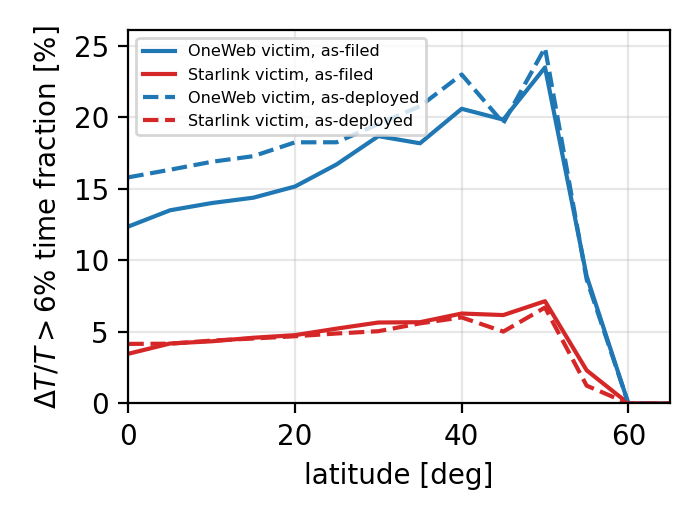
\includegraphics[width=\columnwidth]{B1_events_both.png}
\caption{Realistic-variant $\Delta T/T>\DttThresholdPct\%$ time fraction versus
latitude, both directions, as filed (\EventNPhasings\ phasings) and as deployed
(\NStartTimes\ start times), \EirpHeadDiam~m aperture; per-latitude means over
meridians and replications.}
\label{fig:events}
\end{figure}

\emph{25.261(d) without and with diversity.} All modelled links have baseline
availability of at least \RuleBaselineAvailPct\% (\QualOneCases\ of
\QualOneTotal\ cases qualify). Without diversity, the OneWeb-victim degradation
is \DegrDepMaxPct$\pm$\DegrDepMaxCi\% as deployed and
\DegrFilMaxPct$\pm$\DegrFilMaxCi\% as filed, and the availability change is
\UnavailIncDepPct$\pm$\UnavailIncDepCi\% and \UnavailIncPct$\pm$\UnavailIncCi\%:
both limits are exceeded in both geometries (Fig.~\ref{fig:limits}). With
diversity the degradation falls to \DegrDepDivPct$\pm$\DegrDepDivCi\% and
\DegrFilDivPct$\pm$\DegrFilDivCi\%, and the availability change to
\UnavailDepDivPct\% and \UnavailFilDivPct\%: both limits are met. In the reverse
direction the Starlink-victim degradation is
\DegrDepStarPct$\pm$\DegrDepStarCi\% without diversity, below the limit.

\begin{figure*}[t]
\centering
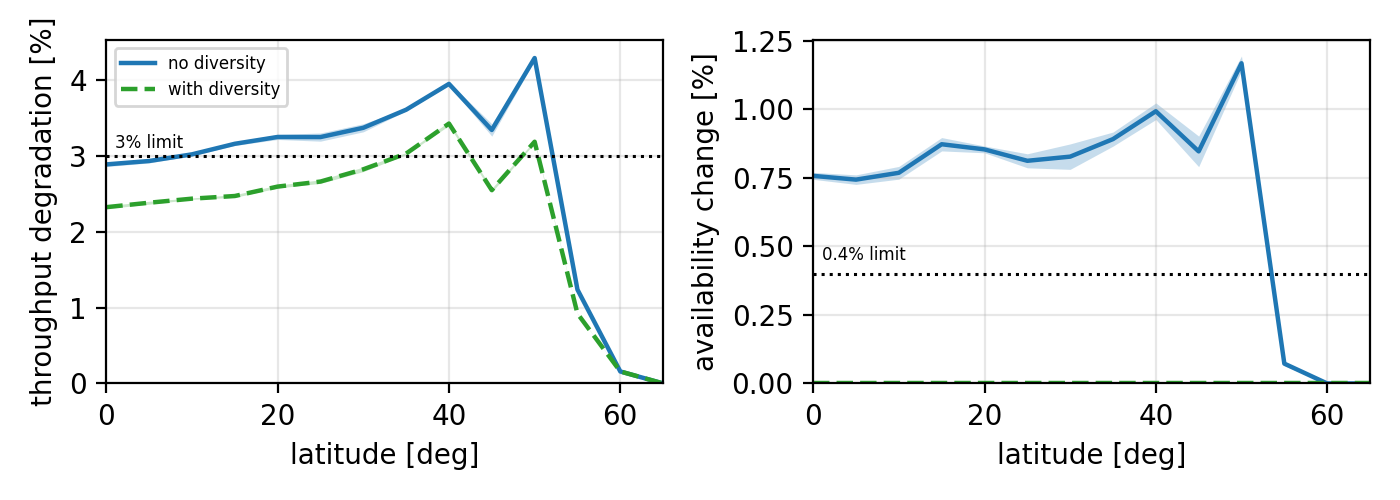
\includegraphics[width=0.8\textwidth]{B2_limits.png}
\caption{\S\,25.261(d) metrics versus latitude, OneWeb victim, realistic variant,
as deployed, \EirpHeadDiam~m: throughput degradation (left) and availability
change (right), without and with diversity; per-latitude means over meridians and
start times. Dotted lines: \DegradeLimitPct\% and \UnavailLimitPct\% limits.}
\label{fig:limits}
\end{figure*}

\emph{Dependence on Starlink power.} Fig.~\ref{fig:pfd} and
Table~\ref{tab:cases} (as deployed, \SenStartTimes\ start times) vary the
interferer power. At the PFD limit both limits are exceeded without diversity
(\TabPrimDegrNoDivPct$\pm$\TabPrimDegrNoDivCi\%,
\TabPrimUnavNoDivPct$\pm$\TabPrimUnavNoDivCi\%), and they remain exceeded
\PfdOffsetThreeDb~dB below it
(\TabPfdMinusThreeDegrNoDivPct$\pm$\TabPfdMinusThreeDegrNoDivCi\%,
\TabPfdMinusThreeUnavNoDivPct$\pm$\TabPfdMinusThreeUnavNoDivCi\%). At
\PfdOffsetSixDb~dB below it the degradation,
\TabPfdMinusSixDegrNoDivPct$\pm$\TabPfdMinusSixDegrNoDivCi\%, meets the limit,
while the availability change,
\TabPfdMinusSixUnavNoDivPct$\pm$\TabPfdMinusSixUnavNoDivCi\%, is not
distinguishable from the \UnavailLimitPct\% threshold. Holding constant EIRP
instead of constant PFD raises the degradation to
\TabConstEirpDegrNoDivPct$\pm$\TabConstEirpDegrNoDivCi\%. The low end of the
filed Starlink range, the del~Portillo common EIRP~\cite{delportillo2019}, and a
OneWeb EIRP calibrated to a C/N target all exceed both limits without diversity.
With diversity, every row meets both limits: the largest degradation is
\TabCnCalDegrDivPct$\pm$\TabCnCalDegrDivCi\% and every availability change is
\TabPrimUnavDivPct\%.

\begin{figure}[t]
\centering
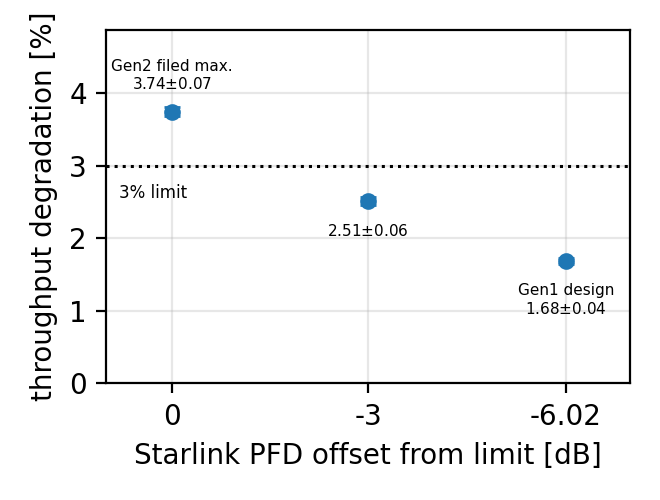
\includegraphics[width=0.86\columnwidth]{B3_pfd_offset.png}
\caption{No-diversity throughput degradation versus Starlink PFD offset from
the 25.208(b) limit, OneWeb victim, realistic, as deployed, \EirpHeadDiam~m;
error bars are \CiPct\% CIs over \SenStartTimes\ start times.}
\label{fig:pfd}
\end{figure}

\begin{table}[t]
\caption{Sensitivity, realistic variant, OneWeb victim, as deployed,
\EirpHeadDiam~m, \SenStartTimes\ start times. Event: worst-station
$\Delta T/T>\DttThresholdPct\%$ fraction; degradation (Degr.) and availability
change (Avail.) as in Section~\ref{sec:model}; ND/D: without/with diversity.
Entries: mean$\pm$\CiPct\% CI, in \%.}
\label{tab:cases}
\centering
\scriptsize
\setlength{\tabcolsep}{1.2pt}
\begin{tabular}{@{}lccccc@{}}
\toprule
Case & Event & Degr.\ ND & Degr.\ D & Avail.\ ND & Avail.\ D\\
\midrule
PFD limit & \TabPrimEventPct$\pm$\TabPrimEventCi
  & \TabPrimDegrNoDivPct$\pm$\TabPrimDegrNoDivCi
  & \TabPrimDegrDivPct$\pm$\TabPrimDegrDivCi
  & \TabPrimUnavNoDivPct$\pm$\TabPrimUnavNoDivCi
  & \TabPrimUnavDivPct$\pm$\TabPrimUnavDivCi\\
Const.\ EIRP & \TabConstEirpEventPct$\pm$\TabConstEirpEventCi
  & \TabConstEirpDegrNoDivPct$\pm$\TabConstEirpDegrNoDivCi
  & \TabConstEirpDegrDivPct$\pm$\TabConstEirpDegrDivCi
  & \TabConstEirpUnavNoDivPct$\pm$\TabConstEirpUnavNoDivCi
  & \TabConstEirpUnavDivPct$\pm$\TabConstEirpUnavDivCi\\
PFD $-\PfdOffsetThreeDb$~dB & \TabPfdMinusThreeEventPct$\pm$\TabPfdMinusThreeEventCi
  & \TabPfdMinusThreeDegrNoDivPct$\pm$\TabPfdMinusThreeDegrNoDivCi
  & \TabPfdMinusThreeDegrDivPct$\pm$\TabPfdMinusThreeDegrDivCi
  & \TabPfdMinusThreeUnavNoDivPct$\pm$\TabPfdMinusThreeUnavNoDivCi
  & \TabPfdMinusThreeUnavDivPct$\pm$\TabPfdMinusThreeUnavDivCi\\
PFD $-\PfdOffsetSixDb$~dB & \TabPfdMinusSixEventPct$\pm$\TabPfdMinusSixEventCi
  & \TabPfdMinusSixDegrNoDivPct$\pm$\TabPfdMinusSixDegrNoDivCi
  & \TabPfdMinusSixDegrDivPct$\pm$\TabPfdMinusSixDegrDivCi
  & \TabPfdMinusSixUnavNoDivPct$\pm$\TabPfdMinusSixUnavNoDivCi
  & \TabPfdMinusSixUnavDivPct$\pm$\TabPfdMinusSixUnavDivCi\\
Starlink low end & \TabLowEventPct$\pm$\TabLowEventCi
  & \TabLowDegrNoDivPct$\pm$\TabLowDegrNoDivCi
  & \TabLowDegrDivPct$\pm$\TabLowDegrDivCi
  & \TabLowUnavNoDivPct$\pm$\TabLowUnavNoDivCi
  & \TabLowUnavDivPct$\pm$\TabLowUnavDivCi\\
del Portillo & \TabDpCommonEventPct$\pm$\TabDpCommonEventCi
  & \TabDpCommonDegrNoDivPct$\pm$\TabDpCommonDegrNoDivCi
  & \TabDpCommonDegrDivPct$\pm$\TabDpCommonDegrDivCi
  & \TabDpCommonUnavNoDivPct$\pm$\TabDpCommonUnavNoDivCi
  & \TabDpCommonUnavDivPct$\pm$\TabDpCommonUnavDivCi\\
OneWeb C/N cal. & \TabCnCalEventPct$\pm$\TabCnCalEventCi
  & \TabCnCalDegrNoDivPct$\pm$\TabCnCalDegrNoDivCi
  & \TabCnCalDegrDivPct$\pm$\TabCnCalDegrDivCi
  & \TabCnCalUnavNoDivPct$\pm$\TabCnCalUnavNoDivCi
  & \TabCnCalUnavDivPct$\pm$\TabCnCalUnavDivCi\\
\bottomrule
\end{tabular}
\end{table}

\emph{Asymmetry.} OneWeb orbits at \OnewebAltKm~km and Starlink at
\StarlinkAltKm~km. As victim, OneWeb receives the PFD-limited signal of the lower,
denser Starlink shell; as interferer, OneWeb's longer slant range and lower EIRP
density weaken its contribution. The burden of both \S\,25.261(c) and
\S\,25.261(d) therefore falls on the higher-altitude, lower-EIRP system.

\section{Limitations}
(a) The S.1528 sidelobe of non-serving interferers assumes nadir-pointing beams.
(b) Consumer terminals are flat panels; the S.1428 dish pattern approximates them.
(c) Each station uses its highest-elevation satellite; operators' selection
policies differ. (d) Diversity is unlimited and assumes knowledge of the
interfering serving satellite; capacity limits would reduce its benefit. (e) Only
the user downlink is modelled. (f) The OneWeb EIRP is taken
from~\cite{delportillo2019}; its constant-EIRP steering and the
\StationMinElevDeg$^\circ$ minimum elevation are assumptions. (g) Starlink is
modelled at the regulatory PFD maximum; Table~\ref{tab:cases} bounds the effect of
lower power. (h) The as-deployed geometry is a single snapshot.

\section{Conclusion}
For the Starlink--OneWeb Ku user downlink, the \S\,25.261 $\Delta T/T$ event is
frequent, peaking at \BindDepWorstPct$\pm$\BindDepWorstCi\% of the time for the
OneWeb victim as deployed, \BurdenRatioDep$\times$ the reverse direction. Without
satellite diversity the \S\,25.261(d) limits are exceeded when Starlink operates at
or near its 25.208(b) PFD limit and still \PfdOffsetThreeDb~dB below it; at
\PfdOffsetSixDb~dB below it the throughput limit is met and the availability
change is not distinguishable from its threshold. With diversity both limits are
met in every case studied. Compliance with \S\,25.261(d) is therefore conditional
on satellite diversity, which the rule neither requires nor credits, and the
burden falls on the higher-altitude, lower-EIRP system.

\bibliographystyle{IEEEtran}
\bibliography{refs}

\end{document}
